\subsubsection{Tổng quan danh mục ADR}

Các quyết định kiến trúc dưới đây được ghi lại để giữ bối cảnh lựa chọn của IRMS, đặc biệt là mối liên hệ giữa yêu cầu phi chức năng ở Mục~\ref{sec:nfr} và các góc nhìn kiến trúc ở Chương~3--4. Phân tích chi tiết vẫn nằm trong thân báo cáo; mỗi ADR chốt một quyết định, trạng thái, căn cứ và hệ quả chính. Các mã ADR được nhắc trong các section chính là liên kết trực tiếp tới bản ghi quyết định tương ứng. Người đọc có thể dùng các liên kết này để xem bối cảnh, căn cứ và hệ quả của từng quyết định kiến trúc.

{\small
\setlength{\LTleft}{0pt}
\setlength{\LTright}{0pt}
\setlength{\tabcolsep}{3pt}
\renewcommand{\arraystretch}{1.12}
\begin{longtable}{@{}>{\raggedright\arraybackslash}p{1.35cm} >{\raggedright\arraybackslash}p{2.35cm} >{\raggedright\arraybackslash}p{4.15cm} >{\raggedright\arraybackslash}p{2.65cm} >{\raggedright\arraybackslash}p{2.75cm}@{}}
\caption{Danh mục quyết định kiến trúc quan trọng của IRMS}\label{tab:adr-catalog}\\
\toprule
\textbf{ADR} & \textbf{Trạng thái} & \textbf{Quyết định} & \textbf{Ý nghĩa kiến trúc} & \textbf{Mục liên kết} \\
\midrule
\endfirsthead
\toprule
\textbf{ADR} & \textbf{Trạng thái} & \textbf{Quyết định} & \textbf{Ý nghĩa kiến trúc} & \textbf{Mục liên kết} \\
\midrule
\endhead
\adrref{ADR-0001}{adr:0001-modular-initial} & Thay thế bởi \adrref{ADR-0002}{adr:0002-service-based} & Modular architecture cho phân rã ban đầu. & Structure, maintainability & Mục~\ref{sec:module-view}. \\
\adrref{ADR-0002}{adr:0002-service-based} & Được chấp nhận; thay thế \adrref{ADR-0001}{adr:0001-modular-initial} & Service-based architecture là kiến trúc chủ đạo; event-driven processing là cơ chế bổ trợ. & Structure, NFR, dependency & Mục~\ref{sec:system-architecture-choice}, Mục~\ref{sec:architecture-overview}. \\
\adrref{ADR-0003}{adr:0003-gateway-boundary} & Được chấp nhận & Gateway boundary cho frontend và REST entry point. & Interface, dependency, security boundary & Mục~\ref{sec:architecture-overview}, Mục~\ref{sec:main-components}. \\
\adrref{ADR-0004}{adr:0004-rest-sync} & Được chấp nhận & REST đồng bộ cho thao tác cần phản hồi trực tiếp. & Interface, responsiveness & Mục~\ref{sec:main-connectors}. \\
\adrref{ADR-0005}{adr:0005-event-driven} & Được chấp nhận & Event-driven processing cho hệ quả bất đồng bộ. & NFR, dependency, scalability & Mục~\ref{sec:connector-rationale}. \\
\adrref{ADR-0006}{adr:0006-outbox} & Được chấp nhận & Outbox pattern để phát event sau giao dịch nghiệp vụ. & Reliability, construction technique & Mục~\ref{sec:connector-rationale}. \\
\adrref{ADR-0007}{adr:0007-rabbitmq} & Được chấp nhận & RabbitMQ làm broker cho luồng event nội bộ. & Dependency, reliability, operation & Mục~\ref{sec:component-connector-view}. \\
\adrref{ADR-0008}{adr:0008-single-postgresql} & Được chấp nhận & Một PostgreSQL vật lý, nhiều nhóm bảng logic. & Data, deployment & Mục~\ref{sec:deployment-view}. \\
\adrref{ADR-0009}{adr:0009-read-model} & Được chấp nhận & Read model logic cho báo cáo. & Data, performance & Mục~\ref{sec:architecture-overview}. \\
\adrref{ADR-0010}{adr:0010-idempotency} & Được chấp nhận & Idempotency/inbox tracking cho consumer nền. & Reliability & Mục~\ref{sec:component-connector-view}. \\
\adrref{ADR-0011}{adr:0011-boundary-adapters} & Được chấp nhận & Boundary adapters cho thanh toán, thông báo và biên nhận. & Interface, extensibility & Mục~\ref{sec:solid-design}. \\
\adrref{ADR-0012}{adr:0012-iam-rbac-audit} & Được chấp nhận & IAM/RBAC và audit log cho thao tác nhạy cảm. & Security, auditability & Mục~\ref{sec:nfr}. \\
\adrref{ADR-0013}{adr:0013-service-layering} & Được chấp nhận & Layering trong từng service. & Structure, maintainability & Mục~\ref{sec:module-view}. \\
\adrref{ADR-0014}{adr:0014-docker-compose} & Được chấp nhận & Docker Compose cho runtime cục bộ. & Deployment, construction & Mục~\ref{sec:deployment-view}. \\
\adrref{ADR-0015}{adr:0015-correlation-id} & Được chấp nhận & Correlation id/logging cho truy vết vận hành. & Observability, auditability & Mục~\ref{sec:nfr}. \\
\bottomrule
\end{longtable}
\normalsize
}

{\small
\setlength{\LTleft}{0pt}
\setlength{\LTright}{0pt}
\setlength{\tabcolsep}{3pt}
\renewcommand{\arraystretch}{1.12}
\begin{longtable}{@{}>{\raggedright\arraybackslash}p{1.35cm} >{\raggedright\arraybackslash}p{3.85cm} >{\raggedright\arraybackslash}p{3.65cm} >{\raggedright\arraybackslash}p{3.95cm}@{}}
\caption{Liên kết ADR với yêu cầu phi chức năng}\label{tab:adr-nfr-links}\\
\toprule
\textbf{ADR} & \textbf{Quyết định} & \textbf{Yêu cầu phi chức năng liên quan} & \textbf{Lý do liên kết} \\
\midrule
\endfirsthead
\toprule
\textbf{ADR} & \textbf{Quyết định} & \textbf{Yêu cầu phi chức năng liên quan} & \textbf{Lý do liên kết} \\
\midrule
\endhead
\adrref{ADR-0001}{adr:0001-modular-initial} & Modular architecture cho phân rã ban đầu. & Bảo trì và mở rộng chức năng. & Tách hệ thống theo vùng nghiệp vụ giúp tổ chức source code dễ hiểu ở giai đoạn đầu. \\
\adrref{ADR-0002}{adr:0002-service-based} & Service-based architecture là kiến trúc chủ đạo. & Khả năng mở rộng; bảo trì; độ phản hồi. & Ranh giới service giúp cô lập thay đổi và mở rộng các vùng tải cao như gọi món, bếp và thanh toán. \\
\adrref{ADR-0003}{adr:0003-gateway-boundary} & Gateway boundary cho frontend. & Bảo trì; quan sát vận hành; bảo mật. & Gateway tạo điểm vào thống nhất để kiểm soát route, lỗi, timeout và chính sách ở biên. \\
\adrref{ADR-0004}{adr:0004-rest-sync} & REST đồng bộ cho thao tác cần phản hồi trực tiếp. & Hiệu năng và độ phản hồi. & Các thao tác tại giao diện phục vụ, bếp và thu ngân cần phản hồi rõ trong thời gian ngắn. \\
\adrref{ADR-0005}{adr:0005-event-driven} & Event-driven processing cho hệ quả bất đồng bộ. & Độ phản hồi; khả năng mở rộng; độ tin cậy. & Báo cáo, thông báo, kiểm toán và cập nhật nền được tách khỏi tuyến giao dịch nóng. \\
\adrref{ADR-0006}{adr:0006-outbox} & Outbox pattern cho event sau giao dịch nghiệp vụ. & Độ tin cậy và toàn vẹn giao dịch. & Ghi event cùng giao dịch nghiệp vụ giúp giảm rủi ro mất event khi publish thất bại. \\
\adrref{ADR-0007}{adr:0007-rabbitmq} & RabbitMQ cho event nội bộ. & Khả năng mở rộng; quan sát vận hành; độ tin cậy. & Broker tách producer khỏi consumer và hỗ trợ xử lý nền độc lập. \\
\adrref{ADR-0008}{adr:0008-single-postgresql} & Một PostgreSQL vật lý, nhiều nhóm bảng logic. & Độ tin cậy; vận hành; bảo trì. & Một database vật lý đơn giản hóa runtime hiện tại, còn module và nhóm bảng giữ ranh giới logic. \\
\adrref{ADR-0009}{adr:0009-read-model} & Read model logic cho báo cáo. & Hiệu năng; khả năng mở rộng; quan sát vận hành. & Truy vấn báo cáo không làm nặng dữ liệu giao dịch chính và có thể chấp nhận độ trễ. \\
\adrref{ADR-0010}{adr:0010-idempotency} & Idempotency/inbox tracking cho consumer nền. & Độ tin cậy và toàn vẹn giao dịch. & Consumer có thể nhận lại event, vì vậy cần tránh xử lý lặp gây tác dụng phụ. \\
\adrref{ADR-0011}{adr:0011-boundary-adapters} & Boundary adapters cho thanh toán, thông báo và biên nhận. & Bảo trì và mở rộng chức năng. & Provider hoặc kênh gửi có thể thay đổi mà không làm service nghiệp vụ phụ thuộc trực tiếp. \\
\adrref{ADR-0012}{adr:0012-iam-rbac-audit} & IAM/RBAC và audit log. & Bảo mật và khả năng kiểm toán. & Hoàn tiền, hủy món, ghi đè giá và thay đổi quyền cần kiểm soát quyền và lưu vết. \\
\adrref{ADR-0013}{adr:0013-service-layering} & Layering trong từng service. & Bảo trì và mở rộng chức năng. & Tách controller, use case, domain policy và adapter hạ tầng giúp giảm trộn trách nhiệm. \\
\adrref{ADR-0014}{adr:0014-docker-compose} & Docker Compose cho runtime cục bộ. & Vận hành; khả năng kiểm thử. & Môi trường cục bộ thống nhất giúp kiểm thử tích hợp và giảm sai lệch cấu hình. \\
\adrref{ADR-0015}{adr:0015-correlation-id} & Correlation id/logging. & Quan sát vận hành; kiểm toán. & Request và event cần truy vết xuyên suốt để phân tích lỗi và đối chiếu thao tác. \\
\bottomrule
\end{longtable}
\normalsize
}

{\small
\setlength{\LTleft}{0pt}
\setlength{\LTright}{0pt}
\setlength{\tabcolsep}{3pt}
\renewcommand{\arraystretch}{1.12}
\normalsize
}

\subsubsection{Nhóm quyết định về phong cách kiến trúc và phân rã}

\paragraph{ADR-0001: Chọn modular architecture cho phân rã ban đầu.}
\label{adr:0001-modular-initial}
\textbf{Trạng thái.} Thay thế bởi \adrref{ADR-0002}{adr:0002-service-based}.

\textbf{Bối cảnh.} Ở giai đoạn đầu, IRMS cần một cách phân rã dễ hiểu để mô tả các vùng nghiệp vụ như đặt bàn, gọi món, bếp, thanh toán, tồn kho, báo cáo, định danh và kiểm toán. Modular architecture phù hợp cho bước khởi đầu vì giúp tách chức năng theo module và tránh trình bày hệ thống như một khối nguyên khối.

\textbf{Quyết định.} Dùng modular architecture/module-based decomposition làm định hướng phân rã ban đầu. Quyết định này chủ yếu phục vụ cấu trúc và tổ chức hiện thực, không còn là phong cách kiến trúc chủ đạo sau khi \adrref{ADR-0002}{adr:0002-service-based} được chấp nhận.

\textbf{Căn cứ.} Quyết định này gắn với yêu cầu bảo trì và mở rộng chức năng ở Mục~\ref{sec:nfr}; hệ thống cần các vùng trách nhiệm đủ rõ để thay đổi thực đơn, giá, tồn kho hoặc báo cáo mà không kéo theo toàn bộ hệ thống.

\begin{figure}[H]
\centering
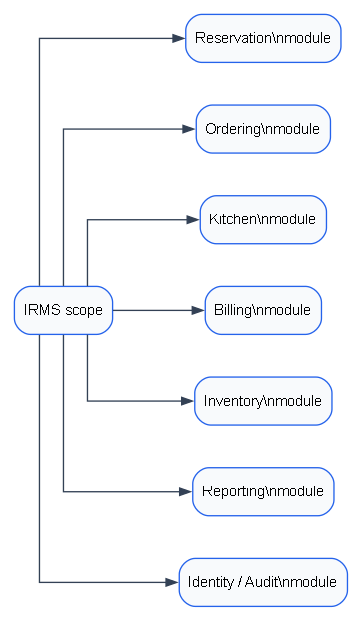
\includegraphics[width=0.78\textwidth,height=0.24\textheight,keepaspectratio]{assets/diagrams/rendered/adr/adr_0001_modular_decomposition.png}
\caption{Minh họa phân rã ban đầu theo module nghiệp vụ của IRMS}
\label{fig:adr-0001-modular}
\end{figure}

\textbf{Hệ quả.}
\begin{itemize}
  \item Module View vẫn hợp lệ để mô tả package, trách nhiệm và phụ thuộc tĩnh.
  \item Cách tiếp cận này chưa đủ để mô tả runtime độc lập, gateway boundary, event/outbox và mở rộng từng vùng chức năng.
  \item \adrref{ADR-0002}{adr:0002-service-based} thay thế quyết định này ở mức architecture style chính, nhưng không phủ nhận giá trị tổ chức module.
\end{itemize}

\textbf{Liên kết với các góc nhìn kiến trúc.} \adrref{ADR-0001}{adr:0001-modular-initial} liên kết trực tiếp với Module View ở Mục~\ref{sec:module-view}; các quyết định runtime được chuyển sang \adrref{ADR-0002}{adr:0002-service-based} và nhóm ADR về giao tiếp.

\paragraph{ADR-0002: Chuyển sang service-based architecture làm kiến trúc chủ đạo.}
\label{adr:0002-service-based}
\textbf{Trạng thái.} Được chấp nhận; thay thế \adrref{ADR-0001}{adr:0001-modular-initial}.

\textbf{Bối cảnh.} Các yêu cầu về mở rộng, phản hồi nhanh, cô lập lỗi, xử lý nền và phối hợp nhiều vùng nghiệp vụ đòi hỏi ranh giới runtime rõ hơn modular architecture ban đầu. IRMS cần giữ tuyến giao dịch nóng ngắn cho gọi món, bếp và thanh toán, trong khi báo cáo, thông báo, kiểm toán và cảnh báo tồn kho có thể xử lý bất đồng bộ.

\textbf{Quyết định.} Chọn service-based architecture làm kiến trúc chủ đạo. Modular decomposition vẫn được giữ trong Module View để tổ chức source code và trách nhiệm module; event-driven processing chỉ là cơ chế bổ trợ cho các hệ quả bất đồng bộ.

\textbf{Căn cứ.} Quyết định này xuất phát từ yêu cầu khả năng mở rộng, độ phản hồi và bảo trì ở Mục~\ref{sec:nfr}, phần lựa chọn kiến trúc ở Mục~\ref{sec:system-architecture-choice} và kiến trúc tổng quan ở Mục~\ref{sec:architecture-overview}.

\begin{figure}[H]
\centering
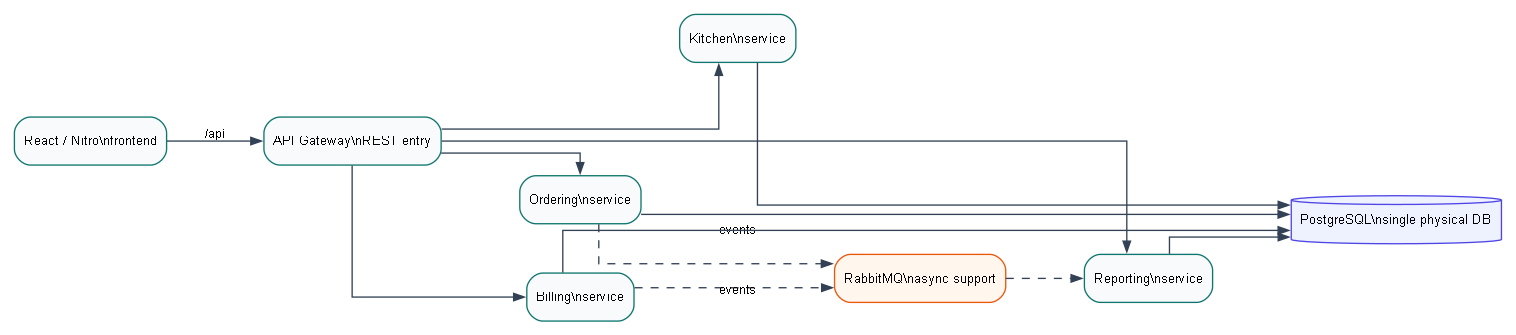
\includegraphics[width=0.82\textwidth,height=0.25\textheight,keepaspectratio]{assets/diagrams/rendered/adr/adr_0002_service_based_architecture.png}
\caption{Minh họa service-based architecture với event-driven processing là cơ chế bổ trợ}
\label{fig:adr-0002-service-based}
\end{figure}

\textbf{Hệ quả.}
\begin{itemize}
  \item Cần quản lý hợp đồng API/event giữa các service.
  \item Gateway boundary, outbox, RabbitMQ và quan sát liên service trở thành quyết định hỗ trợ bắt buộc.
  \item Việc mở rộng từng vùng chức năng khả thi hơn, nhưng làm tăng nhu cầu kiểm soát cấu hình và lỗi liên service.
\end{itemize}

\textbf{Liên kết với các góc nhìn kiến trúc.} \adrref{ADR-0002}{adr:0002-service-based} chi phối kiến trúc tổng quan, Module View và Component-and-Connector View. Deployment View cụ thể hóa quyết định này bằng các runtime service trong Docker Compose.

\paragraph{ADR-0013: Dùng domain/application layering trong từng service.}
\label{adr:0013-service-layering}
\textbf{Trạng thái.} Được chấp nhận.

\textbf{Bối cảnh.} Khi đã dùng service-based architecture, từng service vẫn cần cấu trúc nội bộ đủ rõ để tránh trộn controller, use case, domain policy, repository và adapter hạ tầng. Các package hiện có như \texttt{api}, \texttt{application}, \texttt{domain}, \texttt{infrastructure} và \texttt{integration} thể hiện cách tổ chức theo lớp trong từng miền.

\textbf{Quyết định.} Trong từng service, mã nguồn được tổ chức theo lớp: \texttt{api} tiếp nhận REST, \texttt{application} điều phối use case và port, \texttt{domain} giữ policy/rule, còn \texttt{infrastructure}/\texttt{integration} hiện thực truy cập dữ liệu hoặc kết nối ngoài.

\textbf{Căn cứ.} Quyết định này liên quan trực tiếp đến yêu cầu bảo trì và mở rộng chức năng ở Mục~\ref{sec:nfr}; thay đổi rule nghiệp vụ, adapter hoặc controller cần được khu trú trong lớp đúng vai trò.

\begin{figure}[H]
\centering
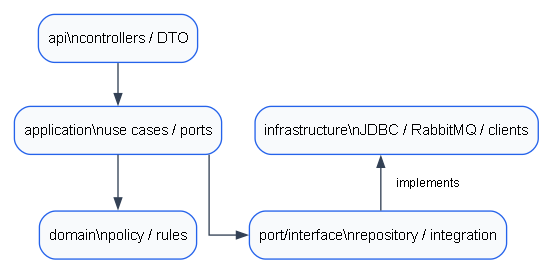
\includegraphics[width=0.62\textwidth,height=0.25\textheight,keepaspectratio]{assets/diagrams/rendered/adr/adr_0013_service_layering.png}
\caption{Minh họa layering trong từng service của IRMS}
\label{fig:adr-0013-layering}
\end{figure}

\textbf{Hệ quả.}
\begin{itemize}
  \item Quy tắc phụ thuộc một chiều cần được giữ ổn định.
  \item Domain policy không nên phụ thuộc trực tiếp vào framework hoặc adapter hạ tầng nếu không cần.
  \item Module View có thể đối chiếu cấu trúc package với trách nhiệm kiến trúc.
\end{itemize}

\textbf{Liên kết với các góc nhìn kiến trúc.} \adrref{ADR-0013}{adr:0013-service-layering} cụ thể hóa Module View và hỗ trợ phần SOLID ở Mục~\ref{sec:solid-design}.

\subsubsection{Nhóm quyết định về giao tiếp runtime}

\paragraph{ADR-0003: Dùng gateway boundary cho frontend và REST entry point.}
\label{adr:0003-gateway-boundary}
\textbf{Trạng thái.} Được chấp nhận.

\textbf{Bối cảnh.} Frontend phục vụ nhiều vai trò vận hành và không nên gọi trực tiếp mọi service nội bộ. Nếu giao diện biết toàn bộ topology backend, thay đổi service URL, port hoặc cấu trúc runtime sẽ lan lên tầng UI.

\textbf{Quyết định.} Frontend đi qua \textsf{Frontend Node Server} và API Gateway; backend dùng \textsf{GatewayProxyController} làm điểm vào REST để định tuyến yêu cầu đến service phù hợp.

\textbf{Căn cứ.} Quyết định này liên quan đến yêu cầu bảo trì, bảo mật và quan sát vận hành ở Mục~\ref{sec:nfr}. Gateway tạo điểm kiểm soát route, lỗi, timeout và chính sách truy cập ở biên hệ thống.

\begin{figure}[H]
\centering
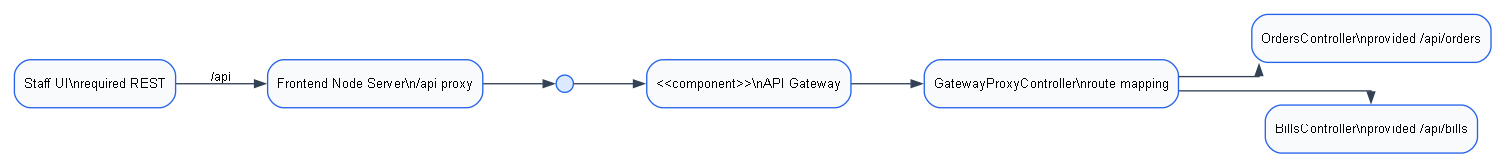
\includegraphics[width=0.78\textwidth,height=0.24\textheight,keepaspectratio]{assets/diagrams/rendered/adr/adr_0003_gateway_boundary.png}
\caption{Minh họa gateway boundary giữa frontend và các REST API nội bộ}
\label{fig:adr-0003-gateway}
\end{figure}

\textbf{Hệ quả.}
\begin{itemize}
  \item Frontend có một entry point ổn định thay vì phụ thuộc trực tiếp vào từng service.
  \item Gateway trở thành điểm cấu hình quan trọng, cần kiểm soát route, timeout và lỗi định tuyến.
  \item Khi gateway lỗi, nhiều luồng nghiệp vụ tuyến đầu có thể bị ảnh hưởng nên healthcheck và log ở biên rất quan trọng.
\end{itemize}

\textbf{Liên kết với các góc nhìn kiến trúc.} \adrref{ADR-0003}{adr:0003-gateway-boundary} liên kết với kiến trúc tổng quan, C\&C View và Deployment View.

\paragraph{ADR-0004: Dùng REST đồng bộ cho thao tác cần phản hồi trực tiếp.}
\label{adr:0004-rest-sync}
\textbf{Trạng thái.} Được chấp nhận.

\textbf{Bối cảnh.} Các thao tác như check-in, tạo order, cập nhật bếp, lập hóa đơn, thanh toán và hoàn tiền cần trả trạng thái thành công/thất bại rõ ràng cho nhân viên. Các thao tác này không phù hợp nếu chỉ phát event rồi chờ xử lý nền.

\textbf{Quyết định.} Dùng REST/API đồng bộ cho thao tác mà người dùng cần phản hồi trực tiếp. Event không thay thế các command tuyến đầu; event chỉ xử lý hệ quả sau khi trạng thái chính đã được ghi nhận.

\textbf{Căn cứ.} Quyết định này liên quan trực tiếp đến yêu cầu hiệu năng và độ phản hồi ở Mục~\ref{sec:nfr}; giao diện phục vụ, bếp và thu ngân cần phản hồi ngắn, nhất quán và dễ hiểu.

\begin{figure}[H]
\centering
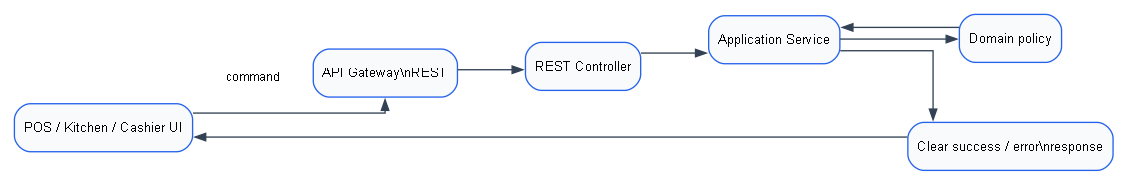
\includegraphics[width=0.78\textwidth,height=0.24\textheight,keepaspectratio]{assets/diagrams/rendered/adr/adr_0004_rest_synchronous.png}
\caption{Minh họa tuyến REST đồng bộ cho command cần phản hồi trực tiếp}
\label{fig:adr-0004-rest}
\end{figure}

\textbf{Hệ quả.}
\begin{itemize}
  \item API contract cần ổn định và phản hồi lỗi phải nhất quán.
  \item Tuyến giao dịch nóng phải ngắn, tránh phụ thuộc vào tác vụ báo cáo hoặc thông báo.
  \item Các thao tác nhạy cảm vẫn cần kiểm quyền và audit theo \adrref{ADR-0012}{adr:0012-iam-rbac-audit}.
\end{itemize}

\textbf{Liên kết với các góc nhìn kiến trúc.} \adrref{ADR-0004}{adr:0004-rest-sync} được thể hiện trong C\&C View, đặc biệt ở phần kiểu kết nối và tuyến lệnh vận hành.

\paragraph{ADR-0005: Dùng event-driven processing cho hệ quả bất đồng bộ.}
\label{adr:0005-event-driven}
\textbf{Trạng thái.} Được chấp nhận.

\textbf{Bối cảnh.} Báo cáo, thông báo, kiểm toán, cập nhật read model và cảnh báo tồn kho là các hệ quả quan trọng nhưng không phải lúc nào cũng cần chặn thao tác chính. Nếu đặt toàn bộ vào giao dịch đồng bộ, các luồng gọi món, bếp và thanh toán sẽ dài hơn và dễ bị nghẽn.

\textbf{Quyết định.} Dùng event-driven processing cho các hệ quả bất đồng bộ sau giao dịch chính. Event-driven processing không phải architecture style chính của IRMS, mà là cơ chế phối hợp hỗ trợ service-based architecture.

\textbf{Căn cứ.} Các yêu cầu về độ phản hồi, khả năng mở rộng và độ tin cậy ở Mục~\ref{sec:nfr} đòi hỏi hệ quả nền không làm dài thao tác tuyến đầu và có thể được xử lý lại khi lỗi.

\begin{figure}[H]
\centering
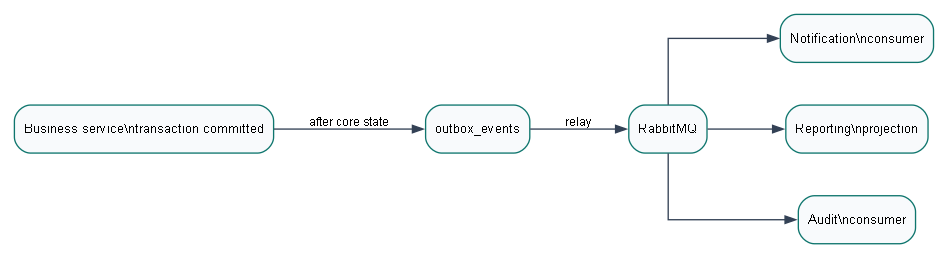
\includegraphics[width=0.78\textwidth,height=0.24\textheight,keepaspectratio]{assets/diagrams/rendered/adr/adr_0005_event_driven_side_effects.png}
\caption{Minh họa event-driven processing cho hệ quả sau giao dịch chính}
\label{fig:adr-0005-event}
\end{figure}

\textbf{Hệ quả.}
\begin{itemize}
  \item Chấp nhận độ trễ có kiểm soát giữa giao dịch chính và hệ quả nền.
  \item Consumer cần idempotency, retry và log đủ để vận hành.
  \item Trạng thái nghiệp vụ tuyến đầu không được phụ thuộc hoàn toàn vào event nền.
\end{itemize}

\textbf{Liên kết với các góc nhìn kiến trúc.} \adrref{ADR-0005}{adr:0005-event-driven} được cụ thể hóa trong Component-and-Connector View và liên kết với \adrref{ADR-0006}{adr:0006-outbox}, \adrref{ADR-0007}{adr:0007-rabbitmq}, \adrref{ADR-0010}{adr:0010-idempotency}.

\paragraph{ADR-0006: Dùng outbox pattern để phát event sau giao dịch nghiệp vụ.}
\label{adr:0006-outbox}
\textbf{Trạng thái.} Được chấp nhận.

\textbf{Bối cảnh.} Khi giao dịch nghiệp vụ đã hoàn tất nhưng bước publish message thất bại, hệ thống có nguy cơ mất event nếu publish trực tiếp. Với các luồng như xác nhận order, thanh toán hoặc cảnh báo tồn kho, mất event có thể làm reporting, notification hoặc audit không đầy đủ.

\textbf{Quyết định.} Event cần phát bất đồng bộ được ghi vào \textsf{outbox\_events} trong cùng transaction với thay đổi nghiệp vụ; sau đó \textsf{RabbitMqOutboxRelay} đọc outbox và publish sang RabbitMQ.

\textbf{Căn cứ.} Yêu cầu độ tin cậy và toàn vẹn giao dịch ở Mục~\ref{sec:nfr} đòi hỏi sự kiện nghiệp vụ không bị mất khi giao dịch chính đã hoàn tất nhưng bước phát thông điệp gặp lỗi.

\begin{figure}[H]
\centering
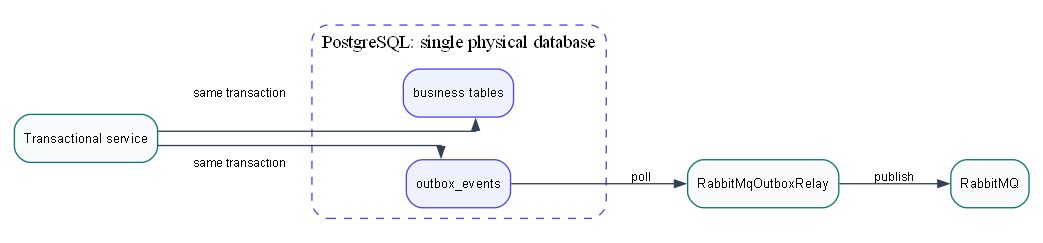
\includegraphics[width=0.78\textwidth,height=0.25\textheight,keepaspectratio]{assets/diagrams/rendered/adr/adr_0006_outbox_pattern.png}
\caption{Minh họa outbox pattern với một PostgreSQL vật lý duy nhất}
\label{fig:adr-0006-outbox}
\end{figure}

\textbf{Hệ quả.}
\begin{itemize}
  \item Cần relay/worker để chuyển event từ outbox sang broker.
  \item Cần quan sát backlog và lỗi publish để tránh event bị kẹt.
  \item \textsf{outbox\_events} là nhóm bảng logic trong cùng PostgreSQL, không phải database riêng.
\end{itemize}

\textbf{Liên kết với các góc nhìn kiến trúc.} \adrref{ADR-0006}{adr:0006-outbox} xuất hiện trong C\&C View, Deployment View và liên kết với \adrref{ADR-0008}{adr:0008-single-postgresql} về dữ liệu.

\paragraph{ADR-0007: Dùng RabbitMQ làm broker cho luồng event nội bộ.}
\label{adr:0007-rabbitmq}
\textbf{Trạng thái.} Được chấp nhận.

\textbf{Bối cảnh.} Các producer như ordering, billing hoặc inventory không nên phụ thuộc trực tiếp vào từng consumer reporting, notification, audit. Broker giúp tách producer khỏi consumer và cho phép các tác vụ nền phát triển độc lập hơn.

\textbf{Quyết định.} Dùng \textsf{RabbitMQ} làm broker cho event nội bộ được phát từ outbox relay đến các consumer nền.

\textbf{Căn cứ.} Quyết định này liên quan đến khả năng mở rộng, độ tin cậy và quan sát vận hành ở Mục~\ref{sec:nfr}; broker hỗ trợ hàng đợi, retry và tách nhịp xử lý giữa producer và consumer.

\begin{figure}[H]
\centering
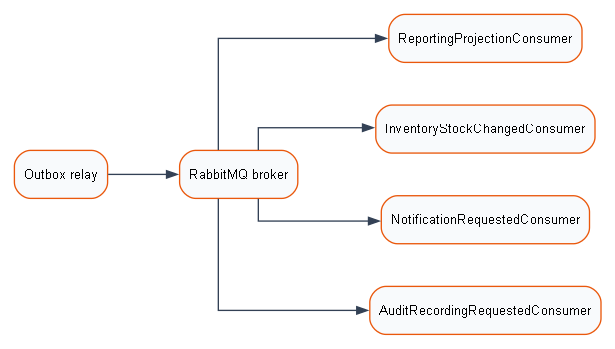
\includegraphics[width=0.78\textwidth,height=0.24\textheight,keepaspectratio]{assets/diagrams/rendered/adr/adr_0007_rabbitmq_broker.png}
\caption{Minh họa RabbitMQ làm broker cho các consumer nền nội bộ}
\label{fig:adr-0007-rabbitmq}
\end{figure}

\textbf{Hệ quả.}
\begin{itemize}
  \item Cần cấu hình broker và theo dõi hàng đợi trong vận hành.
  \item Consumer lỗi không nhất thiết làm sập tuyến giao dịch chính.
  \item Event có thể đến muộn hoặc được gửi lại, nên \adrref{ADR-0010}{adr:0010-idempotency} là điều kiện bổ trợ quan trọng.
\end{itemize}

\textbf{Liên kết với các góc nhìn kiến trúc.} \adrref{ADR-0007}{adr:0007-rabbitmq} nằm trong C\&C View và Deployment View, đồng thời gắn với cấu hình RabbitMQ của runtime Docker.

\subsubsection{Nhóm quyết định về dữ liệu, nhất quán và báo cáo}

\paragraph{ADR-0008: Dùng một PostgreSQL vật lý duy nhất, phân tách theo nhóm bảng logic.}
\label{adr:0008-single-postgresql}
\textbf{Trạng thái.} Được chấp nhận.

\textbf{Bối cảnh.} Phạm vi triển khai hiện tại cần đơn giản, có thể khởi động cục bộ và giữ nhất quán cho giao dịch quan trọng. Tuy nhiên hệ thống vẫn cần phân biệt dữ liệu giao dịch, outbox/inbox, audit, identity/session/policy và read model báo cáo.

\textbf{Quyết định.} Runtime hiện tại chỉ có một \textsf{PostgreSQL} vật lý. Các nhóm \textsf{outbox\_events}, \textsf{processed\_events}, read model, audit và identity/session/policy là nhóm bảng logic trong cùng PostgreSQL.

\textbf{Căn cứ.} Quyết định này liên quan đến độ tin cậy, vận hành và bảo trì ở Mục~\ref{sec:nfr}; một database vật lý đơn giản hóa triển khai, trong khi phân tách logic vẫn giữ được ranh giới trách nhiệm.

\begin{figure}[H]
\centering
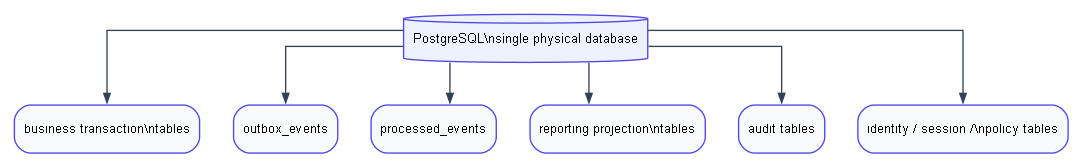
\includegraphics[width=0.62\textwidth,height=0.28\textheight,keepaspectratio]{assets/diagrams/rendered/adr/adr_0008_single_postgresql.png}
\caption{Minh họa một PostgreSQL vật lý duy nhất với nhiều nhóm bảng logic}
\label{fig:adr-0008-postgresql}
\end{figure}

\textbf{Hệ quả.}
\begin{itemize}
  \item Không vẽ hoặc mô tả nhiều database vật lý trong runtime hiện tại.
  \item Cần giữ ranh giới logic qua module, repository, naming và policy truy cập dữ liệu.
  \item Mô hình này phù hợp phạm vi học phần nhưng chưa phải chiến lược database-per-service.
\end{itemize}

\textbf{Liên kết với các góc nhìn kiến trúc.} \adrref{ADR-0008}{adr:0008-single-postgresql} chi phối Deployment View, Data View và các đoạn mô tả read model/outbox trong kiến trúc tổng quan.

\paragraph{ADR-0009: Dùng read model logic cho báo cáo.}
\label{adr:0009-read-model}
\textbf{Trạng thái.} Được chấp nhận.

\textbf{Bối cảnh.} Dashboard và báo cáo quản lý cần truy vấn doanh thu, vận hành, tồn kho và hiệu suất mà không làm nặng tuyến giao dịch chính. Báo cáo có thể chấp nhận độ trễ có kiểm soát nếu đổi lại thao tác gọi món, bếp và thanh toán ổn định hơn.

\textbf{Quyết định.} Reporting dùng read model/projection tables trong cùng PostgreSQL để phục vụ dashboard và báo cáo. Projection được cập nhật qua event hoặc tiến trình nền, không được mô tả như một database vật lý riêng.

\textbf{Căn cứ.} Quyết định này liên quan đến hiệu năng, khả năng mở rộng và quan sát vận hành ở Mục~\ref{sec:nfr}; truy vấn báo cáo không nên tranh chấp trực tiếp với dữ liệu giao dịch nóng.

\begin{figure}[H]
\centering
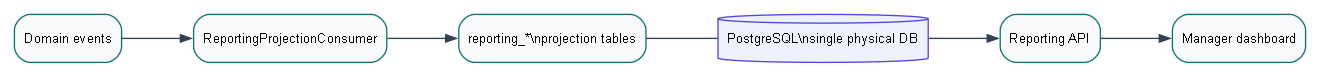
\includegraphics[width=0.78\textwidth,height=0.24\textheight,keepaspectratio]{assets/diagrams/rendered/adr/adr_0009_read_model_reporting.png}
\caption{Minh họa read model báo cáo là nhóm bảng logic trong cùng PostgreSQL}
\label{fig:adr-0009-read-model}
\end{figure}

\textbf{Hệ quả.}
\begin{itemize}
  \item Dữ liệu báo cáo có thể trễ so với giao dịch gốc.
  \item Cần mô tả rõ read model là projection logic, không phải reporting database riêng.
  \item Khi event hoặc consumer lỗi, dashboard có thể chậm cập nhật nhưng không nên chặn tuyến giao dịch chính.
\end{itemize}

\textbf{Liên kết với các góc nhìn kiến trúc.} \adrref{ADR-0009}{adr:0009-read-model} liên kết với kiến trúc tổng quan, C\&C View xử lý nền và các activity/reporting use case.

\paragraph{ADR-0010: Dùng idempotency/inbox tracking cho consumer nền.}
\label{adr:0010-idempotency}
\textbf{Trạng thái.} Được chấp nhận.

\textbf{Bối cảnh.} Event delivery có thể retry hoặc trùng. Nếu consumer inventory, reporting, notification hoặc audit xử lý lặp mà không kiểm soát, hệ thống có thể ghi nhận sai projection, gửi thông báo lặp hoặc tạo audit không nhất quán.

\textbf{Quyết định.} Consumer nền ghi nhận event đã xử lý thông qua \textsf{processed\_events} hoặc cơ chế tương đương trước/sau khi xử lý theo contract của consumer. Khi nhận event đã xử lý, consumer bỏ qua hoặc xử lý theo nhánh an toàn.

\textbf{Căn cứ.} Quyết định này liên quan trực tiếp đến yêu cầu độ tin cậy và toàn vẹn giao dịch ở Mục~\ref{sec:nfr}; các luồng nền không được gây tác dụng phụ lặp khi event được gửi lại.

\begin{figure}[H]
\centering
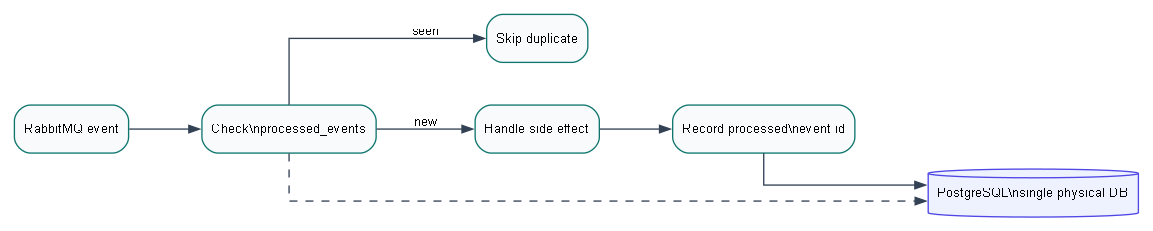
\includegraphics[width=0.78\textwidth,height=0.24\textheight,keepaspectratio]{assets/diagrams/rendered/adr/adr_0010_idempotent_consumers.png}
\caption{Minh họa kiểm tra \textsf{processed\_events} để tránh xử lý event lặp}
\label{fig:adr-0010-idempotency}
\end{figure}

\textbf{Hệ quả.}
\begin{itemize}
  \item Consumer cần định danh event ổn định và kiểm tra trạng thái đã xử lý.
  \item Cần quan sát lỗi consumer và event bị retry nhiều lần.
  \item \textsf{processed\_events} là nhóm bảng logic trong cùng PostgreSQL.
\end{itemize}

\textbf{Liên kết với các góc nhìn kiến trúc.} \adrref{ADR-0010}{adr:0010-idempotency} cụ thể hóa phần xử lý nền trong C\&C View và hỗ trợ \adrref{ADR-0005}{adr:0005-event-driven}, \adrref{ADR-0007}{adr:0007-rabbitmq}.

\subsubsection{Nhóm quyết định về bảo mật, mở rộng và triển khai}

\paragraph{ADR-0011: Dùng boundary adapters cho thanh toán, thông báo và biên nhận.}
\label{adr:0011-boundary-adapters}
\textbf{Trạng thái.} Được chấp nhận.

\textbf{Bối cảnh.} Thanh toán, thông báo và phát hành biên nhận là các điểm dễ thay đổi theo chính sách vận hành hoặc kênh tích hợp. Lõi nghiệp vụ không nên phụ thuộc trực tiếp vào provider cụ thể, đặc biệt khi phạm vi hiện tại chỉ thể hiện adapter nội bộ.

\textbf{Quyết định.} Các kênh thanh toán, thông báo và biên nhận đi qua port/interface như \textsf{PaymentGateway}, \textsf{NotificationChannelAdapter} và \textsf{ReceiptDeliveryAdapter}.

\textbf{Căn cứ.} Quyết định này liên quan trực tiếp đến yêu cầu bảo trì và mở rộng chức năng ở Mục~\ref{sec:nfr}; khi thêm phương thức thanh toán hoặc kênh thông báo mới, thay đổi cần khu trú ở adapter và kiểm thử contract.

\begin{figure}[H]
\centering
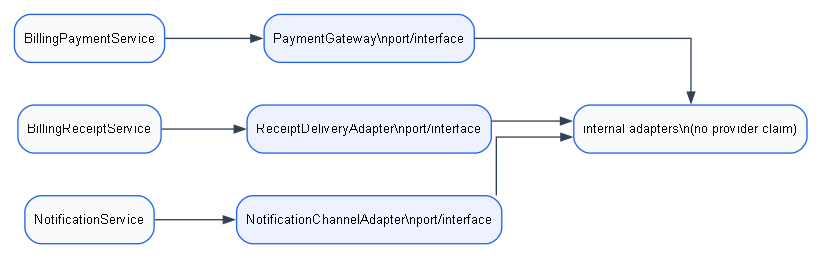
\includegraphics[width=0.78\textwidth,height=0.24\textheight,keepaspectratio]{assets/diagrams/rendered/adr/adr_0011_boundary_adapters.png}
\caption{Minh họa boundary adapters cho thanh toán, thông báo và biên nhận}
\label{fig:adr-0011-adapters}
\end{figure}

\textbf{Hệ quả.}
\begin{itemize}
  \item Service nghiệp vụ phụ thuộc vào contract ổn định thay vì provider cụ thể.
  \item Cần kiểm thử contract cho từng adapter.
  \item Không trình bày như đã tích hợp provider thanh toán/SMS/email ngoài nếu phạm vi hiện tại chỉ có adapter nội bộ.
\end{itemize}

\textbf{Liên kết với các góc nhìn kiến trúc.} \adrref{ADR-0011}{adr:0011-boundary-adapters} liên kết với Class Diagram, C\&C View và phần SOLID ở Mục~\ref{sec:solid-design}.

\paragraph{ADR-0012: Dùng IAM/RBAC và audit log cho thao tác nhạy cảm.}
\label{adr:0012-iam-rbac-audit}
\textbf{Trạng thái.} Được chấp nhận.

\textbf{Bối cảnh.} Hoàn tiền, hủy món đã gửi bếp, ghi đè giá, thay đổi quyền, điều chỉnh tồn kho và truy cập audit log là các thao tác nhạy cảm. Hệ thống cần kiểm soát ai được thực hiện thao tác nào và lưu vết đủ để đối chiếu sau vận hành.

\textbf{Quyết định.} Dùng IAM/RBAC tại lớp định danh và lớp biên; kết hợp \textsf{AuthorizationPolicy} cho điều kiện nghiệp vụ; ghi \textsf{AuditLog} hoặc audit event cho thao tác nhạy cảm.

\textbf{Căn cứ.} Yêu cầu bảo mật và kiểm toán ở Mục~\ref{sec:nfr} quy định các thao tác nhạy cảm phải kiểm soát vai trò, ghi nhận người thực hiện, thời điểm, giá trị và lý do khi cần.

\begin{figure}[H]
\centering
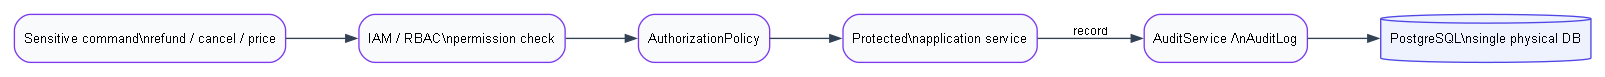
\includegraphics[width=0.78\textwidth,height=0.24\textheight,keepaspectratio]{assets/diagrams/rendered/adr/adr_0012_iam_rbac_audit.png}
\caption{Minh họa kiểm quyền và audit log cho thao tác nhạy cảm}
\label{fig:adr-0012-iam-audit}
\end{figure}

\textbf{Hệ quả.}
\begin{itemize}
  \item Kiểm quyền không chỉ nằm ở gateway mà còn cần xuất hiện ở quy tắc nghiệp vụ.
  \item Audit là luồng bắt buộc cho thao tác nhạy cảm.
  \item Cần giữ user context và correlation id để truy vết đầy đủ.
\end{itemize}

\textbf{Liên kết với các góc nhìn kiến trúc.} \adrref{ADR-0012}{adr:0012-iam-rbac-audit} liên kết với yêu cầu phi chức năng, kiến trúc tổng quan, class identity/audit và các activity diagram quản trị.

\paragraph{ADR-0014: Dùng Docker Compose cho runtime cục bộ và trình bày học phần.}
\label{adr:0014-docker-compose}
\textbf{Trạng thái.} Được chấp nhận.

\textbf{Bối cảnh.} IRMS cần môi trường có thể khởi động nhất quán để kiểm thử tích hợp và trình bày chức năng. Runtime hiện tại gồm frontend, API gateway, các service Spring Boot, PostgreSQL, RabbitMQ và migration container.

\textbf{Quyết định.} Dùng \textsf{Docker Compose} để khởi động local runtime gồm app services, PostgreSQL, RabbitMQ và migration.

\textbf{Căn cứ.} Quyết định này liên quan đến yêu cầu vận hành và khả năng kiểm thử ở Mục~\ref{sec:nfr}; Compose giúp giảm sai lệch cấu hình giữa các lần chạy và làm rõ thứ tự khởi động.

\begin{figure}[H]
\centering
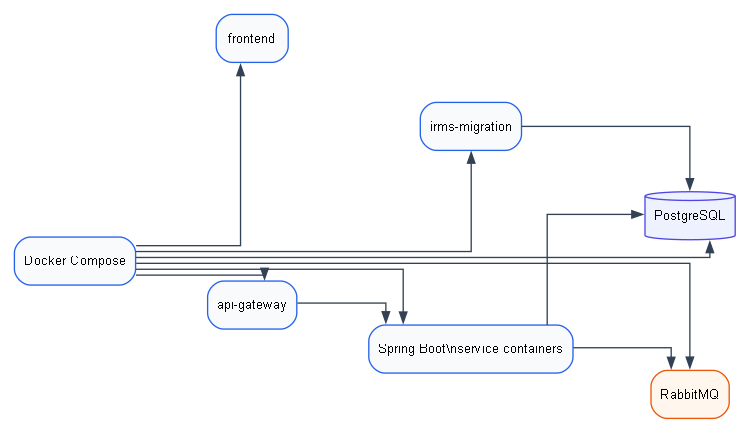
\includegraphics[width=0.82\textwidth,height=0.25\textheight,keepaspectratio]{assets/diagrams/rendered/adr/adr_0014_docker_compose_runtime.png}
\caption{Minh họa runtime Docker Compose cục bộ của IRMS}
\label{fig:adr-0014-compose}
\end{figure}

\textbf{Hệ quả.}
\begin{itemize}
  \item Compose phù hợp kiểm thử tích hợp và demo trong phạm vi học phần.
  \item Không mô tả load balancer, replica hoặc production cluster như cấu hình đã triển khai nếu chưa có căn cứ.
  \item Migration cần chạy trước các service nghiệp vụ để schema nhất quán.
\end{itemize}

\textbf{Liên kết với các góc nhìn kiến trúc.} \adrref{ADR-0014}{adr:0014-docker-compose} liên kết với Deployment View, Install View và Phụ lục hướng dẫn chạy project.

\paragraph{ADR-0015: Dùng centralized logging/correlation id cho truy vết vận hành.}
\label{adr:0015-correlation-id}
\textbf{Trạng thái.} Được chấp nhận.

\textbf{Bối cảnh.} Các yêu cầu ghi dữ liệu, event nền, hoàn tiền, kiểm toán và báo cáo cần truy vết xuyên suốt từ request ban đầu đến service và consumer liên quan. Nếu thiếu correlation id, việc điều tra lỗi hoặc đối chiếu audit sau ca vận hành sẽ khó hơn.

\textbf{Quyết định.} Các request/event quan trọng mang correlation id để truy vết qua gateway, application service, event metadata, consumer và audit/log.

\textbf{Căn cứ.} Quyết định này liên quan đến yêu cầu khả năng quan sát và vận hành ở Mục~\ref{sec:nfr}; report và thiết kế hiện tại đã mô tả correlation id như một phần của dữ liệu giao dịch, event metadata và audit context.

\begin{figure}[H]
\centering
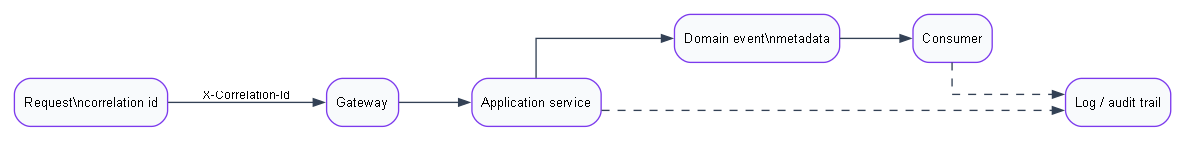
\includegraphics[width=0.78\textwidth,height=0.24\textheight,keepaspectratio]{assets/diagrams/rendered/adr/adr_0015_correlation_id.png}
\caption{Minh họa correlation id đi qua request, service, event và audit/log}
\label{fig:adr-0015-correlation}
\end{figure}

\textbf{Hệ quả.}
\begin{itemize}
  \item REST request và event cần truyền correlation id nhất quán.
  \item Audit/log cần giữ correlation id để đối chiếu sau vận hành.
  \item Nếu mở rộng observability sau này, correlation id là nền tảng cho tracing đầy đủ hơn.
\end{itemize}

\textbf{Liên kết với các góc nhìn kiến trúc.} \adrref{ADR-0015}{adr:0015-correlation-id} liên kết với C\&C View, yêu cầu phi chức năng về quan sát vận hành và các luồng audit trong thiết kế chi tiết.

Các bản ghi ADR được lưu cùng tài liệu dự án trong thư mục \texttt{docs/adr}.
